\documentclass[a4paper,14pt]{extarticle}

\usepackage[a4paper,top=20mm,bottom=20mm,left=30mm,right=10mm]{geometry}
\usepackage[T1,T2A]{fontenc}
\usepackage[utf8]{inputenc}
\usepackage[russian]{babel}
\usepackage{indentfirst}
\usepackage{titlesec}
\usepackage{graphicx}
\usepackage{verbatim}
\usepackage{fancyvrb}
\usepackage{hyperref}

\renewcommand{\baselinestretch}{1.3}

\titleformat{\section}{\normalsize\bfseries}{\thesection}{1em}{}
\titleformat{\subsection}{\normalsize\bfseries}{\thesubsection}{1em}{}

\setlength{\parindent}{12.5mm}

\begin{document}

\newpage\thispagestyle{empty}
\begin{center}
  \MakeUppercase{
    Министерство науки и высшего образования Российской Федерации\\
    Федеральное государственное бюджетное образовательное учреждение высшего образования\\
    <<Вятский Государственный Университет>>\\
  }
  Институт математики и информационных систем\\
  Факультет автоматики и вычислительной техники\\
  Кафедра электронных вычислительных машин
\end{center}
\vfill

\begin{center}
  Отчет по лабораторной работе №1\\
  по дисциплине\\
  <<Объектно-ориентированное программирование>>\\
\end{center}
\vfill

\noindent
\begin{tabular}{ll}
  Выполнил студент гр. ИВТб-2301-05-00 \hspace{5mm} & \rule[-1mm]{25mm}{0.10mm}\,/Макаров С.А./ \\
  Руководитель преподаватель                        & \rule[-1mm]{25mm}{0.10mm}\,/Шмакова Н.А./ \\
\end{tabular}

\vfill
\begin{center}
  Киров 2026
\end{center}

\newpage
\section*{\hspace{12.5mm}Цель работы}
Цель работы: изучить и освоить принципы объектно-ориентированного программирования, включая инкапсуляцию, наследование и полиморфизм, путем создания иерархии классов в выбранной предметной области.

\section*{\hspace{12.5mm}Задание}
\begin{enumerate}
  \item Создать иерархию классов состоящую не менее чем из одного родительского  и двух дочерних классов.
  \item В каждом классе определить не менее  двух член данных. не менее двух собственных, а для дочерних не менее двух унаследованных и двух перекрытых член функций.
  \item Разработать приложение демонстрирующее принципы инкапсуляции, наследования и полиморфизма.
\end{enumerate}

\section*{\hspace{12.5mm}Решение}
Предметная область описывает управление ассортиментом блюд в заведении общественного питания. Система позволяет хранить информацию о различных блюдах, учитывать их специфические характеристики, рассчитывать итоговую цену для клиента в зависимости от этих характеристик и выводить информацию о блюде в удобном виде.

Программа содержит классы <<Dish>>, представлющий базовый класс блюда,  <<Pizza>>, наследованный от <<Dish>> и представлющий класс пиццы, <<Salad>> наследованный от <<Dish>> и представлющий класс салата.

Базовый класс <<Dish>> содержит:
\begin{itemize}
  \item[--] Поля:
  \begin{itemize}
    \item[--] private std::string name -- приватное поле, означающее название блюда, строковый тип данных;
    \item[--] private int weight -- приватное поле, означающее вес блюда, целочисленный тип данных;
    \item[--] private double price -- приватное поле, цена блюда, формат с плавающей запятой;
  \end{itemize}
  \item[--] Конструкторы:
  \begin{itemize}
    \item[--] public Dish() - публичный конструктор, задает значения полей по умолчанию;
    \item[--] public Dish(std::string name) - публичный конструктор, принимает название блюда в качестве параметра;
    \item[--] public Dish(std::string name, int weight, double price) - публичный конструктор, принимает  в качестве параметров название, вес и цену блюда;
  \end{itemize}
  \item[--] Геттеры/сеттеры:
  \begin{itemize}
    \item[--] public std::string GetName() const -- геттер, возвращает название блюда;
    \item[--] public int GetWeight() const -- геттер, возвращает вес блюда;
    \item[--] public double GetPrice() const -- геттер, возвращает цену блюда;
    \item[--] public void SetName(std::string name) -- сеттер, задает значение названию блюда, принимает в качестве параметра название блюда;
    \item[--] public void SetWeight(int weight) -- сеттер, задает значение весу блюда, принимает в качестве параметра вес блюда;
    \item[--] public void SetPrice(double price) -- сеттер, задает значение цене блюда, принимает в качестве параметра цену блюда;
  \end{itemize}
  \item[--] Абстрактные методы:
  \begin{itemize}
    \item[--] public virtual void DisplayInfo() = 0 -- публичный виртуальный метод, отображающий информацию о блюде, не принимает параметров;
    \item[--] public virtual double CalcFullPrice() = 0 -- публичный виртуальный метод, возвращающий полную цену блюда.
  \end{itemize}
\end{itemize}

Класс <<Pizza>>, наследованный от класса <<Dish>> содержит:
\begin{itemize}
  \item[--] Собственные поля:
  \begin{itemize}
    \item[--] private Dough dough = Dough::Thick -- приватное поле, означающее типа теста, по умолчанию Thick;
  \end{itemize}
  \item[--] Конструкторы:
  \begin{itemize}
    \item[--] public Pizza() : Dish() -- публичный конструктор, задает значения полей по умолчанию;
    \item[--] public Pizza(std::string name) : Dish(name) -- публичный конструктор, принимает название пиццы в качестве параметра;
    \item[--] public Pizza(std::string name, int weight, double price) : Dish(name, weight, price) -- публичный конструктор, принимает в качестве параметров название, вес и цену пиццы;
  \end{itemize}
  \item[--] Геттеры/сеттеры:
  \begin{itemize}
    \item[--] public Dough GetDough() const -- геттер, возвращает тип теста;
    \item[--] public void SetDough(Dough dough) -- сеттер, задает значение типу теста, принимает в качестве параметра enum Dough (Thick, Thin);
  \end{itemize}
  \item[--] Переопределенные методы:
  \begin{itemize}
    \item[--] public void DisplayInfo() override -- публичный метод, отображает информацию о пицце (название, тип теста, вес, цена), не принимает параметров, выводит информацию в следующем виде:
    \begin{Verbatim}[tabsize=4]
Pizza: Margarita, thick dough, 450g, $18.00;
    \end{Verbatim}
    \item[--] public double CalcFullPrice() override -- публичный метод, возвращает полную цену в зависимости от типа теста (Thick: price * 1.5, Thin: price * 1.3), не принимает параметров;
  \end{itemize}
  \item[--] Собственные методы:
  \begin{itemize}
    \item[--] public void ChangeDough() -- публичный метод, меняет тип теста, не принимает параметров;
    \item[--] public void CutInSlices() -- публичный метод, нарезает пиццу на куски, не принимает параметров, выводит информацию в следующем виде:
    \begin{Verbatim}[tabsize=4]
Cutting the pizza into slices...;
    \end{Verbatim}
  \end{itemize}
\end{itemize}

Класс <<Salad>>, наследованный от класса <<Dish>> содержит:
\begin{itemize}
  \item[--] Собственные поля:
  \begin{itemize}
    \item[--] private Dressing dressing -- приватное поле, означающее приватное поле, о тип заправки, по умолчанию OliveOil;
  \end{itemize}
  \item[--] Конструкторы:
  \begin{itemize}
    \item[--] public Salad() : Dish() -- публичный конструктор, задает значения полей по умолчанию;
    \item[--] public Salad(std::string name) : Dish(name) -- публичный конструктор, принимает название салата в качестве параметра;
    \item[--] public Salad(std::string name, int weight, double price) : Dish(name, weight, price) -- публичный конструктор, принимает в качестве параметров название, вес и цену салата;
  \end{itemize}
  \item[--] Геттеры/сеттеры:
  \begin{itemize}
    \item[--] public Dressing GetDressing() const -- геттер, возвращает тип заправки;
    \item[--] public SetDressing(Dressing dressing) -- сеттер, задает значение типу заправки, принимает в качестве параметра enum Dressing (OliveOil, Mayonnaise);
  \end{itemize}
  \item[--] Переопределенные методы:
  \begin{itemize}
    \item[--] public void DisplayInfo() override -- публичный метод, отображает информацию о салате (название, тип заправки, вес, цена), не принимает параметров,  информацию в следующем виде:
    \begin{Verbatim}[tabsize=4]
Salad: Caesar, OliveOil dressing, 250g, $12.60;
    \end{Verbatim}
    \item[--] public double CalcFullPrice() override -- публичный метод, возвращает полную цену в зависимости от типа заправки (OliveOil: price * 1.4, Mayonnaise: price * 1.3), не принимает параметров
  \end{itemize}
  \item[--] Собственные методы:
  \begin{itemize}
    \item[--] public void ChangeDressing() -- публичный метод, меняет тип заправки, не принимает параметров;
    \item[--] public void TossWithDressing() -- публичный метод, перемешивает салат с заправкой, не принимает параметров, выводит информацию в следующем виде:
    \begin{Verbatim}[tabsize=4]
Tossing the salad with OliveOil...;
    \end{Verbatim}
  \end{itemize}
\end{itemize}

Диаграмма классов представлена на рисунке 1.

\begin{figure}[ht]
  \centering
  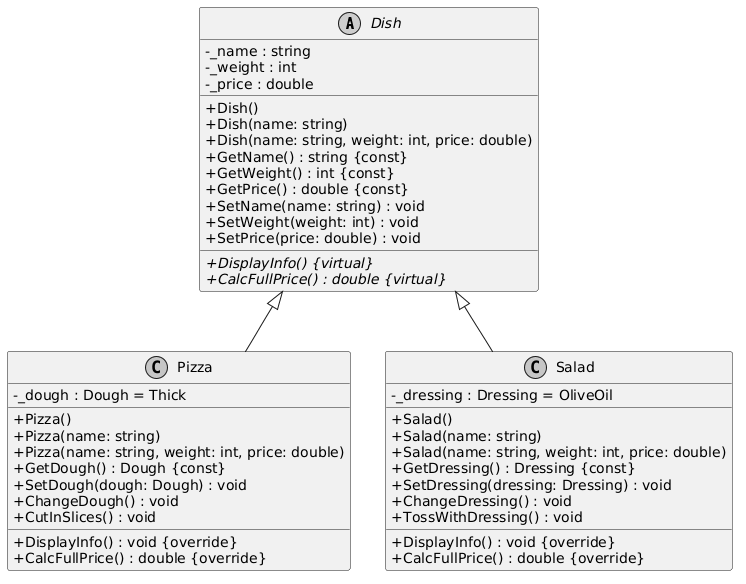
\includegraphics[width=1\linewidth]{img/uml.png}
\end{figure}
\begin{center}
  Рисунок 1 – Диаграмма классов
\end{center}

\section*{\hspace{12.5mm}Вывод}
В ходе выполнения лабораторной работы была разработана и реализована иерархия классов, моделирующая управление ассортиментом блюд в заведении общественного питания. Изучены основные принципы объектно-ориентированного программированя: инкапсуляция, наследование, полиморфизм. Разработано приложение, демонстрирующее применение данных принципов.

\end{document}